\section{Análisis del estado de máxima entropía}

\subsection{Separabilidad}
Una pequeña manipulación de la ecuación (\ref{eq:MaxEntLagMult}),nos permite ver que el argumento de la exponencial se comporta de dos operadores que conmutan entre sí. A notar que
\begin{align*}
    \sum_{i}\lambda_{i}\hat{G}_{i}=&\sum_{i}\lambda_{i}(p\pauli{i}\otimes\Id+(1-p)\Id\otimes\pauli{i})\\
    =&p\sum_{i}\lambda_{i}\pauli{i}\otimes\Id+(1-p)\sum_{i}\lambda_{i}\Id\otimes\pauli{i}\\
    =&p\qty(\sum_{i}\lambda_{i}\pauli{i})\otimes\Id+(1-p)\Id\otimes\qty(\sum_{i}\lambda_{i}\pauli{i}).
\end{align*}
Por supuesto, los operadores 
\begin{align*}
    \qty(\sum_{i}\lambda_{i}\pauli{i})\otimes\Id && \text{y} && \Id\otimes\qty(\sum_{i}\lambda_{i}\pauli{i})
\end{align*} 
conmutan entre sí, así que la exponencial de la ecuación (\ref{eq:MaxEntLagMult}) se puede separar, quedando
\begin{align*}
    \varrho_{\max}=&\frac{1}{Z}e^{\qty(\sum_{i}\lambda_{i}\pauli{i})\otimes\Id }e^{\Id\otimes\qty(\sum_{i}\lambda_{i}\pauli{i})}\\
    &=\frac{1}{Z}e^{p\sum_{i}\lambda_{i}\pauli{i}}\otimes e^{(1-p)\sum_{i}\lambda_{i}\pauli{i}}.
\end{align*}
Hemos obtenido, de esta forma, la expresión separable del estado de máxima entropía,
\begin{equation}\label{eq:MaxEntSeparable}
    \varrho_{\max}=\frac{e^{p\sum_{i}\lambda_{i}\sigma_{i}}}{Z_{1}} \otimes \frac{e^{(1-p)\sum_{i}\lambda_{i}\sigma_{i}}}{Z_{2}}.
\end{equation}

Un resultado así puede parecer demasiado sencillo, y puede propiciar preguntas como: ¿qué significa que el estado de máxima entropía sea separable? ¿Qué interpretación tienen las matrices de densidad reducidas del estado de máxima entropía? Pues bien, primero hace falta ver que la información accesible al experimentalista no incluye las correlaciones entre los subsistemas. Si queda alguna duda sobre esto, considérese la parametrización de Bloch de un estado fino $\varrho\in\mcL(\hilbert_{4})$ como propuesta en (\ref{eq::BlochParametrization4}). La acción de la aplicación sobre la matriz de densidad es
\begin{align*}
    \CG{\varrho}&=\CG{\frac{1}{4}\sum_{i,j=0}^{3}\gamma_{ij}\pauli{i}\otimes \pauli{j}}\\
    &=\frac{1}{2}\qty(\Id+\sum_{k=1}^{3}(p\gamma_{k,0}+(1-p)\gamma_{0,k})\sigma_{k}).
\end{align*}
De esto nos damos cuenta que a través de la aplicación de grano grueso se pierden todas las correlaciones, pues estas corresponden a las componentes $\gamma_{i,j}$ con $i,j\in\{1,2,3\}$. Por la construcción de la aplicación de grano grueso, cualquier sistema de matrices de densidad reducidas $\rho_{A}$ y $\rho_{B}$ da como resultado el mismo estado efectivo, sin importar qué tan factorizable o entrelazado esté (de nuevo, siempre y cuando las marices de densidad reducidas sean $\rho_{A}$ y $\rho_{B}$, pues un sistema máximamente entrelazado arroja como ambas trazas parciales al estado máximamente mezclado). Pues bien, como estas correlaciones se pierden a la hora de hacer las mediciones, en el estado de máxima entropía estas se hacen cero, ya que no se hace ninguna suposición al respecto. 

La expresión (\ref{eq:MaxEntSeparable}) es un producto tensorial de dos operadores de densidad, a los que denotaremos como $\rho_{A}$ y $\rho_{B}$, con $\rho_{A}, \rho_{B}\in\mcL(\hilbert_{2})$. Aún más, nótese que ambos factores pueden reescribirse como la exponencial real de un vector de Pauli $\lambda\paulivec{\lambda}$ con $\hat{\lambda}_{i}=\frac{\lambda_{i}}{\lambda}$ pesado por un factor probabilístico. Ahora, en virtud de la relación (\ref{ap:PauliRealExp}) hallamos
\begin{align*}
    \rho_{A}=\frac{1}{Z_{1}}\qty(\Id\cosh{p\lambda}+\paulivec{\lambda}\sinh{p\lambda}), && \rho_{B}=\frac{1}{Z_{2}}\qty(\Id\cosh{(1-p)\lambda}+\paulivec{\lambda}\sinh{(1-p)\lambda})\rlap{.}
\end{align*}
Para que ambas matrices reducidas representen estados válidos, las funciones de partición $Z_{1}$ y $Z_{2}$ deben valer
\begin{align*}
    2\cosh{p\lambda} && \text{y} && 2\cosh{(1-p)\lambda}
\end{align*}
respectivamente. Las matrices de densidad reducidas del estado de máxima entropía tienen la forma
\begin{align}
    \rho_{A}=\frac{1}{2}\qty(\Id+\paulivec{\lambda}\tanh{p\lambda}) && \text{y} && \rho_{B}=\frac{1}{2}\qty(\Id+\paulivec{\lambda}\tanh{(1-p)\lambda})\rlap{.}
\end{align}

\subsection{La relación entre multiplicadores y mediciones}


El problema de la ecuación (\ref{eq:MaxEntSeparable}) es que el estado de máxima entropía está en términos de los multiplicadores de Lagrange, en lugar de cantidades medibles. Si por alguna razón tuviéramos que resignarnos a trabajar con el estado en términos de los $\lambda_{i}$, será necesario conocer la expresión del estado macroscópico. Para hallarla, basta con pasar al estado de máxima entropía por la aplicación de grano grueso. Por contrucción 
\begin{equation*}
    \rho=\frac{1}{Z}\CG{\varrho_{max}}=p\rho_{A}+(1-p)\rho_{B}.
\end{equation*}
Sustiyendo las fórmulas de $\rho_{A}$ y $\rho_{B}$, obtenemos al estado grueso en términos de los multiplicadores de Lagrange.
\begin{equation}\label{eq:CG(MaxEnt)}
  \rho=\frac{1}{2}[\Id+(\paulivec{\lambda})(p\tanh{\lambda p}+(1-p)\tanh{\lambda (1-p)})].
\end{equation}
Pues bien, el estado efectivo tiene su propia parametrización de Bloch, y es
\begin{equation}\label{eq:EffectiveState}
    \rho=\frac{1}{2}(\Id+r_{\rho}\paulivec{r}).
\end{equation}
Si se comparan las ecuaciones (\ref*{eq:CG(MaxEnt)}) y (\ref*{eq:EffectiveState}), se verá que es posible expresar la pureza $\purity{\rho}$ en términos de $\lambda$. Esto es importante porque la pureza del estado es una cantidad que se puede calcular a través de los valores esperados de los tres observables $\pauli{i}$, según $\text{Pu}(\rho)=\frac{1}{2}(r_{\rho}^{2}+1)$. Definiendo
\begin{equation}\label{eq:r(lambda)}
    \rfroml(\lambda)=p\tanh{\lambda p}+(1-p)\tanh{\lambda (1-p)}
\end{equation}
obtenemos tanto el radio del vector de Bloch del estado en términos de $\lambda$,
\begin{equation*}
    r_{\rho}=\rfroml(\lambda),
\end{equation*}
así como su dirección,
\begin{equation*}
    \hat{r}_{\rho}=\hat{\lambda}.
\end{equation*}
Con estas dos ecuaciones deducimos la relación entre las cantidades medibles $\expval{\pauli{i}}=r_{\rho}(\hat{r}_{\rho})_{i}$ y los multiplicadores de Lagrange introducidos para la maximización de la entropía, y es
\begin{equation}
    \expval{\pauli{i}}=\rfroml(\lambda)(\hat{\lambda})_{i}.
\end{equation}
La función $\rfroml$ es precisamente la hallada en (\ref{eq:MaxEntExpVals}). Ahora, la ecuación (\ref{eq:r(lambda)}), fijada $p$, es una suma de dos funciones inyectivas, y como tal, es inyectiva también. Esto significa que existe la función inversa. La figura \ref{fig:r(lambda)} muestra la forma de $\rfroml(\lambda)$ para valores selectos de $p$. Después de una breve inspección de (\ref{eq:r(lambda)}) se concluyen las siguientes cosas:
\begin{itemize}
\item la superficie es simétrica respecto al plano $p=0.5$
\item los estados puros corresponden al caso límite $\lambda\rightarrow+\infty$
\end{itemize}
\begin{figure}[ht]
    \centering
    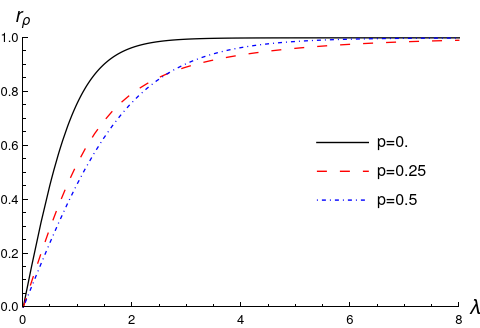
\includegraphics[width=0.6\linewidth]{chapter2/figures/r(lambda).png}
    \caption{$r_{\rho}$ como función de $\lambda$ para diferentes valores de $p$}
    \label{fig:r(lambda)}
\end{figure}
Cada multiplicador de Lagrange queda determinado de forma única a través de cantidades experimentales según 
\begin{equation}
    \lambda_{i}=\rfroml^{-1}(r_{\rho}) \frac{\expval{\pauli{i}}}{r_{\rho}},
\end{equation}
y, por supuesto,
\begin{equation*}
    \lambda=\rfroml^{-1}(r_{\rho})
\end{equation*}
Aunque siempre exista, no es posible hallar una expresión de $\rfroml^{-1}$ para cualquier valor de $p$ debido a que la ecuación (\ref{eq:r(lambda)}) es una ecuación trascendental. Por esto, para escribir al estado de máxima entropía como una función de cantidades medibles, nos tendremos que conformar con llamar a $\rfroml^{-1}$ de manera explícita.

\subsubsection{Dos soluciones particulares}

Hay al menos dos casos en las que $\rfroml^{-1}$ tiene una expresión sencilla. Primero, considerando el caso $p=0$ o $p=1$, la ecuación (\ref{eq:r(lambda)}) se reduce a 
\begin{align*}
\rfroml(\lambda)=&\tanh{\lambda}\\
\Rightarrow\rfroml^{-1}(r_{\rho})=&\text{arctanh}(r_{\rho}).
\end{align*}
Luego, si $p=\frac{1}{2}$, la ecuación (\ref{eq:r(lambda)}) se reduce a
\begin{align*}
    \rfroml(\lambda)=&\tanh{\frac{1}{2}\lambda}\\
    \Rightarrow\rfroml^{-1}(r_{\rho})=&2\text{arctanh}(r_{z}).
\end{align*}

\subsection{Otra expresión del estado de máxima entropía}

La ecuación (\ref{eq:MaxEntSeparable}) sugiere que el estado de máxima entropía puede expresarse como producto tensorial de potencias de un mismo estado. En efecto,
\begin{align*}
  \varrho_{\max}=&\frac{e^{p\sum_{i}\lambda_{i}\pauli{i}}}{Z_{1}} \otimes \frac{e^{(1-p)\sum_{i}\lambda_{i}\pauli{i}}}{Z_{2}}\\
  =&\frac{\qty(e^{\sum_{i}\lambda_{i}\pauli{i}})^{p} }{Z_{1}}\otimes \frac{\qty(e^{\sum_{i}\lambda_{i}\pauli{i}})^{1-p}}{Z_{2}}\\
  =&\frac{\qty(e^{\lambda(\paulivec{r_{\rho}})})^{p}}{Z_{1}} \otimes \frac{\qty(e^{\lambda(\paulivec{r_{\rho}})})^{1-p}}{Z_{2}}.
\end{align*}
En virtud de (\ref*{ap:PauliRealExp}), se cumple que
\begin{align*}
  \varrho_{\max}=&\frac{\qty(\cosh{\lambda}(\Id+\tanh{\lambda}(\paulivec{r_{\rho}})))^{p}}{\Tr[\qty(\cosh{\lambda}(\Id+\tanh{\lambda}(\paulivec{r_{\rho}})))^{p}]} \otimes \frac{\qty(\cosh{\lambda}(\Id+\tanh{\lambda}(\paulivec{r_{\rho}})))^{1-p}}{\Tr[\qty(\cosh{\lambda}(\Id+\tanh{\lambda}(\paulivec{r_{\rho}})))^{1-p}]}\\
  =&\frac{\qty(\Id+\tanh{\lambda}(\paulivec{r_{\rho}}))^{p}}{\Tr[\qty(\Id+\tanh{\lambda}(\paulivec{r_{\rho}}))^{p}]} \otimes \frac{\qty(\Id+\tanh{\lambda}(\paulivec{r_{\rho}}))^{1-p}}{\Tr[\qty(\Id+\tanh{\lambda}(\paulivec{r_{\rho}}))^{1-p}]}.
\end{align*}
Definimos
\begin{equation}\label{eq:Xi}
  \Xi_{\max}=\frac{1}{2}(\Id+\tanh{\lambda}(\paulivec{r_{\rho}})).
\end{equation}
de tal manera que 
\begin{equation}\label{eq:MaxEntSeparablePower}
  \varrho_{\max}=\frac{(\Xi_{\max})^{p}}{\Tr[ (\Xi_{\max})^{p}]}\otimes\frac{(\Xi{\max})^{1-p}}{\Tr[(\Xi_{\max})^{1-p}]}
\end{equation}

\subsection{Generalización: N a M sistemas de dos niveles}

\subsubsection{De n qubits a un qubit}
La discusión anterior giró alrededor del caso en que el modelo de grano grueso reduce un espacio de dos qubits a uno de un solo qubit. Esto puede generalizarse al caso en que el aparato de medición sólo detecta una partícula cuando el sistema microscópico comporta $n$ partículas. En particular, consideramos, nuevamente, subsistemas de dos niveles (qubits), de tal forma que $\varrho\in\densityspace{2}^{\otimes n}$. Primero, veamos que la aplicación de grano grueso que resuelve un qubit donde hay $n$ qubits se puede escribir como
\begin{equation*}
    \CG{\varrho}=\Tr_{\overline{i}}(\Fuzzy{\varrho})=\Tr^{1}(\Fuzzy{\varrho}).
\end{equation*}
Sin pérdida de generalidad, y donde $\Tr_{\overline{i}}$ denota la traza parcial sobre todos menos el $i$-ésimo qubit. La aplicación borrosa permuta el primer qubit con el $j$-ésimo qubit con probabilidad $p_{j}$. Denotando las matrices de permutación como $S_{1,j}$,
\begin{equation*}
    \CG{\varrho}=\Tr_{\overline{1}}\qty(p_{1}\varrho+\sum_{j=2}^{n}p_{j}(S_{1,j})\varrho(S_{1,j})^{\dagger}).
\end{equation*}
Sea $\{A_{i}\}$ con $A_{i}\in\mcL(\hilbert_{2})$ un conjunto de observables tomográficamente completo. Las restricciones a las que se verá sujeto el operador $\varrho_{\max}$ son
\begin{equation*}
    r_{i}=\Tr[\sigma_{i}\rho].
\end{equation*}
Como antes, las restricciones parecen estar definidas en un espacio diferente al del estado microscópico, pero las podemos expresar en términos de operadores que actúan sobre $\hilbert_{2}^{\otimes n}$ como
\begin{align*}
    r_{i}&=\Tr[\sigma_{i}\CG{\varrho}]\\
    &=\Tr[\sigma_{i}\Tr_{\overline{1}}\qty(p_{1}\varrho+\sum_{j=2}^{n}p_{j}(S_{1,j})\varrho(S_{1,j})^{\dagger})]\\
    &=\Tr[\sigma_{i}\otimes\Id_{2^{n-1}}\qty(p_{1}\varrho+\sum_{j=2}^{n}p_{j}(S_{1,j})\varrho(S_{1,j})^{\dagger})]\\
    &=\Tr[\qty(p_{1}(\sigma_{i}\otimes\Id_{2^{n-1}})+\sum_{j=2}^{n}p_{j}(S_{1,j})^{\dagger}(\sigma_{i}\otimes\Id_{2^{n-1}})(S_{1,j}))\varrho]\\
    &=\Tr[\qty(p_{1}(\sigma_{i}\otimes\Id_{2^{n-1}})+\sum_{j=2}^{n}p_{j}(\Id_{2^{j-1}}\otimes\sigma_{i}\otimes\Id_{2^{n-j}}))\varrho]\\
    &=\Tr[\qty(\sum_{j=1}^{n}p_{j}(\Id_{2^{j-1}}\otimes\sigma_{i}\otimes\Id_{2^{n-j}}))\varrho].
\end{align*}
Si definimos
\begin{equation}\label{eq:GhatNM}
    \hat{G}_{i}=\sum_{j=1}^{n}p_{j}(\Id_{2^{j-1}}\otimes\sigma_{i}\otimes\Id_{2^{n-j}}),
\end{equation}
las restricciones experimentales leen
\begin{equation}\label{eq:MaxEntRestrictionsNM}
    r_{i}=\Tr[\hat{G}_{i}\varrho].
\end{equation}
El estado que máximiza la entropía y satisface las restricciones anteriores es
\begin{equation}\label{eq:MaxEntLagMultNM}
    \varrho_{max}(\rho)=\frac{1}{Z}e^{-\sum_{i}\lambda_{i}\hat{G}_{i}}.
\end{equation}
Nuevamente, el argumento de la exponencial puede verse como una suma de $n$ operadores que conmuntan entre sí. Esto significa que el estado de máxima entropía es separable y tiene exactamente $n$ factores. Explícitamente,
\begin{equation}
    \rho_{max}=\Motimes_{j=1}^{n}\frac{1}{Z_{j}}\text{exp}\qty(-p_{j}\sum_{i}\lambda_{i}\sigma_{i}).
\end{equation}

\subsubsection{De N qubits a M qubits}\label{subsec:ch2NM}
\notaAd{
La siguiente extensión corresponde al caso en que detectamos $M$ qubits en lugar de $N$, con $M<N$. Una diferencia inmediata al caso $M=1$ es que, por tener acceso a las correlaciones entre $M$ de las $N$ partículas, el estado que maximiza la entropía no es necesariamente separable.
Primero, utilizamos la aplicación borrosa que permuta cada una de las primeras $M$ partículas con las otras $N-1$. Esta aplicación tiene la forma
\begin{equation*}
    \Fuzzy{\varrho}=p_{0}\varrho+\sum_{m=1}^{M}\sum_{n=m+1}^{N}p_{m,n}(S_{m,n})\varrho(S_{m,n})^{\dagger}.
\end{equation*}
Luego, la herramienta de medición detecta únicamente $M$ partículas, y denotamos esto como $\Tr_{\overline{M}}$. El modelo de grano grueso Es
\begin{equation*}
    \CG{\varrho}=\Tr_{\overline{M}}\qty(p_{0}\varrho+\sum_{m=1}^{M}\sum_{n=m+1}^{N}p_{m,n}(S_{m,n})\varrho(S_{m,n})^{\dagger})
\end{equation*}

Asumiendo que tenemos acceso a un conjunto tomográficamente completo de $m^{2}-1$ observables, $\{A_{i}\}$ con $A_{i}\in\mcL(\hilbert_{2}^{\otimes m})$, podemos hallar las restricciones del estado de máxima entropía compatible. Una posible elección de estos observables son los productos tensoriales de los operadores de Pauli,
\begin{equation*}
    A_{\vec{v}}=\pauli{v_{1}}\otimes\pauli{v_{2}}\otimes...\otimes\pauli{v_{m}}
\end{equation*}
donde las entradas $v_{i}$ del vector $\vec{v}$ toman valores 0, 1, 2, 3.
Las restricciones a las que se verá sujeto el operador $\varrho_{\max}$ son
\begin{equation*}
    \expval{A_{\vec{v}}}=Tr(\pauli{v_{1}}\otimes\pauli{v_{2}}\otimes...\otimes\pauli{v_{n}}\rho)
\end{equation*}
Para traducir estas restricciones al espacio $\densityspace{2}^{\otimes N}$,
\begin{align*}
    &=\Tr[A_{\vec{v}}\mcC(\varrho)]\\
    &=\Tr[A_{\vec{v}}\Tr_{\overline{M}}\qty(p_{0}\varrho+\sum_{m=1}^{M}\sum_{n=m+1}^{N}p_{m,n}(S_{m,n})\varrho(S_{m,n})^{\dagger})]\\
    &=\Tr[A_{\vec{v}}\otimes\Id_{2^{n-m}}\qty(p_{0}\varrho+\sum_{m=1}^{M}\sum_{n=m+1}^{N}p_{m,n}(S_{m,n})\varrho(S_{m,n})^{\dagger})]\\
    &=\Tr[\qty(p_{0}(A_{\vec{v}}\otimes\Id_{2^{n-m}})+\sum_{m=1}^{M}\sum_{n=m+1}^{N}p_{m,n}(S_{m,n})^{\dagger}(A_{\vec{v}}\otimes\Id_{2^{n-m}})(S_{m,n}))\varrho].
\end{align*}
}
\acnote{Aquí me quedé, no sé si deba dejar esto. Además, y ahora que lo pienso, no sé bien ni qué se debe permutar con qué}